\section{Requirements Specification and Security Risk Management}
Security Concerns/Goals: 
\begin{itemize}
	\item Vertraulichkeit (erreichbar durch Kryptographie)\\
	nicht mehr gewährleistet, wenn vertrauliche Informationen von unautorisierten veröffentlicht werden (Bsp: Private Key verloren)
	\item Integrität (erreichbar durch Kryptographie)\\
	= Verhinderung unautorisierter Modifikation von Daten\\
	Datenintegrität und Quellintegrität
	\item Verfügbarkeit\\
	beinhaltet zusichern von zeitlichem und verfügbarem Zugriff auf Informationen
\end{itemize}
Zugriffskontrolle beinhaltet sowohl Authentisierung (etwas beglaubigen) als auch Authentifizierung (sich ggüber Server ausweisen)\\
denken wie die 'bösen Buben' ({\tiny really?! irgendwie kommt mir der ganze Lehrstuhl vor wie im Kindergarten...})\\
\textbf{Computersicherheit} = Schutz der aufgebracht wird um die drei Security Concerns bei einem System zu erhalten\\
\textbf{Authentizität} = Echtheit, Überprüfbarkeit einer Eigenschaft/User\\
\textbf{Veratwortlichkeit} = Zuordnung von Aktionen zu Usern/Dateien etc\\
\\
\textbf{Security Bruch}\\
3 Level
\begin{itemize}
	\item \textbf{Low Impact}: nur geringe/begrenzte Auswirkungen..
	\item \textbf{Moderate Impact}: signifikante Auswirkungen..
	\item \textbf{High Impact}: starke/ernste Auswirkungen..
\end{itemize}
.. auf Gewinn, Individuen etc\\
\\
\textbf{Security Requirements  - Beispiele:}\\
\textit{Studenten - Vertraulichkeit}
\begin{itemize}
	\item Hohe Vertraulichkeit: die Noten selber - Einsicht nur von Studenten und einigen Mitarbeitern, die damit arbeiten müssen
	\item Moderate Vertraulichkeit: Immatrikulation
	\item Geringe Vertraulichkeit: Inhaltsverzeichnis = Studentenliste, Fakultätsliste; published on Website etc
\end{itemize}

\textit{Patienteninformationen - Integrität}
\begin{itemize}
	\item Hohe Integrität: medizinische Unterlagen; sind sie falsch könnte eine falsche Behandlung angewandt werden
	\item Moderate Integrität: Website für Diskussionen von med. Themen
	\item Niedrige Integrität: anonyme Umfragen (zB Patientenzufriedenheit)
\end{itemize}

\textit{Verfügbarkeit - je kritischer eine Komponente, desto höher muss die Verfügbarkeit sein}
\begin{itemize}
	\item Hohe Verfügbarkeit: Authentifizierungsservice (if Service nicht erreichbar, dann restliche Funktionalität auch nicht)
	\item Moderate Verfügbarkeit: College Web Site
	\item Niedrige Verfügbarkeit: Online Phone Directory
\end{itemize}

\subsection{Security Attacks}
\begin{itemize}
	\item Störung/Unterbrechen: Angriff auf Verfügbarkeit\\
	Traffic stören; physisch Leitungen durchtrennen
	\item Abhören: Angriff auf Vertraulichkeit\\
	Mitschneiden von Kommunikation
	\item Modifikation: Angriff auf Integrität\\
	Verändern der Daten bevor sie Ziel erreichen
	\item Fälschen: Angriff auf Authentizität\\
	Daten fälschen; sich als jemand anderes ausgeben
\end{itemize}

\begin{figure}[!h]
	\centering
	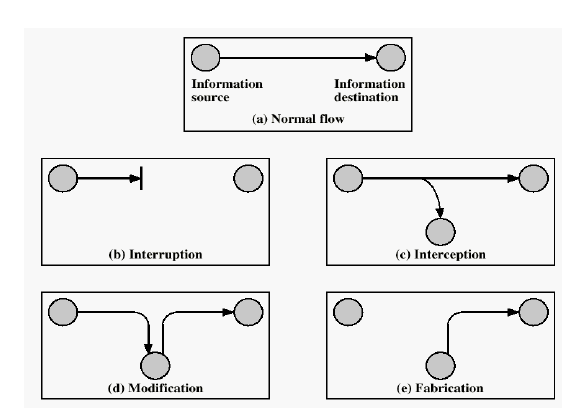
\includegraphics[scale=0.6]{img/security_attacks.png}
	\caption{Flow bei Angriffen}
\end{figure}

\subsection{Bedrohung bekämpfen}
Eine mögliche Vorgehensweise:
\begin{enumerate}
	\item Identify assets (Vermögen?)
	\item Document Architecture
	\item Anwendung zerlegen
	\item Bedrohungen identifizieren
	\item Bedrohungen dokumentieren
	\item Bedrohungen bewerten
\end{enumerate}

\textbf{Kategorisierung von Bedrohungen - STRIDE}
\begin{itemize}
	\item \textbf{Spoofing} Angreifer mit falscher Identität erhält Zugriff
	\item \textbf{Tampering (Manipulation)} Kann Angreifer Daten manipulieren?
	\item \textbf{Repudiation (Ablehnung)} Angreifer verneint Ausnutzen einer Sicherheitslücke. Kann man dies widerlegen?
	\item \textbf{Information Disclosure (Datenenthüllung)} Kann Angreifer an private Daten kommen?
	\item \textbf{DoS}
	\item \textbf{Elevation of Privilege} Kann Angreifer privilegierten Nutzer identifizieren?
\end{itemize}

\textbf{Wichtigkeit von Bedrohungen - DREAD}
\begin{itemize}
	\item \textbf{Damagepotenial} Was sind die Auswirkungen eines exploits?
	\item \textbf{Reproducibility (Reproduzierbarkeit)} Funktioniert der Exploit immer oder nur unter bestimmten Umständen?
	\item \textbf{Exploitability} Skills des Angreifers gut oder schlecht?
	\item \textbf{Affected Users (Betroffene User)} Wie viele User sind betroffen?
	\item \textbf{Discoverability (Entdeckbarkeit)} Wie wahrscheinlich ist die Entdeckung eines Exploits?
\end{itemize} 

\textbf{Risikobewältigung VS. Risikobwertung}
\begin{table}[!h]
	\begin{tabular}{|l|l|l|}
		\hline
				& \textbf{Risikobewältigung}	& \textbf{Risikobewertung}\\
		\hline
		\textbf{Ziel}	& Risiko auf ein akzeptables Lvl reduzieren & Identifizieren und Priorisieren des Risikos\\
		\hline
		\textbf{Cycle} 	& durch alle 4 Phasen\ref{risk_management}	& extra Phase dafür\\
		\hline
		\textbf{Schedule} & festgesetzte Aktivität & fortwährende Aktivität\\
		\hline
		\textbf{Alignment} & angepasst an Budget der jeweiligen Phase & nicht anwendbar \\
		\hline
	\end{tabular}
\end{table}
\begin{figure}[!h]
	\centering
	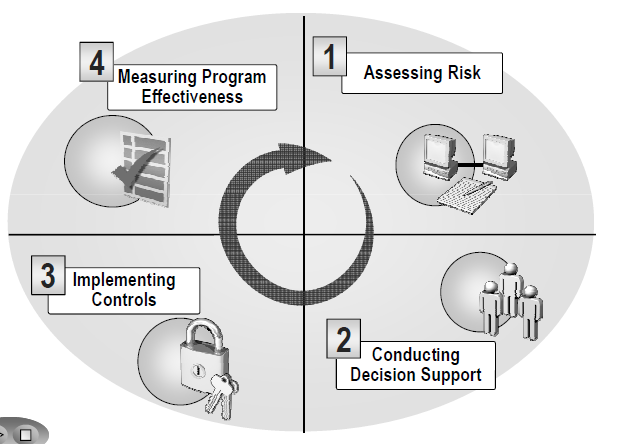
\includegraphics[scale=0.7]{img/risk_management.png}
	\caption{Risikobewältigung}
	\label{risk_management}
\end{figure}
\textbf{Risikobewältigungsphasen}
\begin{enumerate}
	\item Risikobewertung\\
	Risikodaten sammeln; Priorisieren des Risikos
	\item Unterstützungen für Entscheidungen aufstellen; Quasi Risikopläne aufstellen und Kosten dafür
	\begin{enumerate}
		\item def. functional R
		\item Identify Kontrolllösungen
		\item Abgleich Lösung gg R
		\item Grad der Risikoreduktion bewerten
		\item Kosten jeder Lösung bestimmen
		\item Strategie asuwählen
	\end{enumerate}
	\item Kontrollmechanismen implementieren
	\item Messen der Programmeffizienz
\end{enumerate}

\begin{figure}[!h]
	\centering
	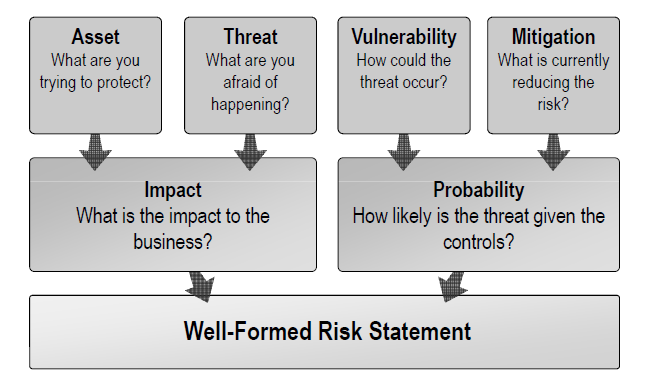
\includegraphics[scale=0.7]{img/comm_risk.png}
	\caption{Risiko kommunizieren}
\end{figure}

\newpage
\subsection{Threat Modeling - Bedrohungen modellieren}
\textbf{Ziele}
\begin{itemize}
	\item Identifizieren wo Anwendung am verwundbarsten
	\item Bestimme Bedrohungen, die eine Abschwächung benötigen (= die bekämpft werden müssen?)
	\item Reduziere Risiko auf akzeptables Lvl durch Abschwächung
\end{itemize}

Kurzer Thread Modeling Process
\begin{enumerate}
	\item Bestimmte Kernszenarios
	\item Modelliere Anwendung mit Data Flow Diagrams
	\item Bestimmte Bedrohungen für jedes DFD
	\item Berechne Risiko
	\item Plane Abschwächung
\end{enumerate}

\begin{figure}[!h]
	\centering
	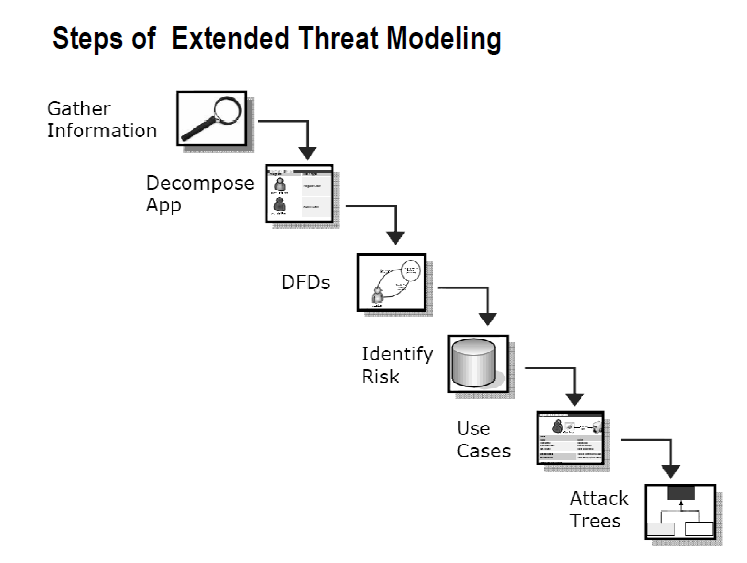
\includegraphics[scale=0.7]{img/extended_thread_modeling.png}
	\caption{Erweitertes Thread Modeling}
\end{figure}
